\documentclass[A4paper,12pt]{article}
\usepackage[utf8]{inputenc} % set input encoding (not needed with XeLaTeX)
\usepackage[title]{appendix}
\usepackage[T1]{fontenc}
\usepackage[stable]{footmisc}
\usepackage{amsmath}
\usepackage{lipsum}
\usepackage{mathtools,amssymb}
\usepackage[margin=1.1in]{geometry} % to change the page dimensions
\usepackage{graphicx} % support the \includegraphics command and options
\usepackage{cancel}
\usepackage{booktabs} % for much better looking tables
\usepackage{array} % for better arrays (eg matrices) in maths
\usepackage{paralist} % very flexible & customisable lists (eg. enumerate/itemize, etc.)
\usepackage{verbatim} % adds environment for commenting out blocks of text & for better verbatim
\usepackage{multirow}
\usepackage{rotating}
\usepackage{pdflscape}
\usepackage{lscape}
\usepackage{tabularx}
\usepackage{booktabs}
\usepackage{amsthm}
\usepackage{setspace}
\usepackage{amssymb,mathtools,amsthm,mathrsfs}
\usepackage{graphicx} 
\usepackage{caption} 
\usepackage{subcaption}
\usepackage{bm}
\usepackage{bbm}
\usepackage{float}
\usepackage{xcolor}
\usepackage{hyperref}
\hypersetup{colorlinks,linkcolor={red!50!black},citecolor={blue!80!black},urlcolor={blue!80!black}}
\usepackage{adjustbox}
%\usepackage{pdfpages}
\usepackage{dsfont}
\usepackage{adjustbox} %RT
\usepackage{threeparttable}
\usepackage[toc,page]{appendix}
\usepackage{mathptmx}
\usepackage[final]{pdfpages}
\usepackage[backend=biber,style=apa]{biblatex}
\usepackage{dcolumn}
\usepackage[verbose]{placeins}
\addbibresource{references.bib}
\newcolumntype{C}{>{\centering\arraybackslash}p{3.5em}}

% Allow line breaks with \\ in special cells
\newcommand{\specialcell}[2][c]{%
\begin{tabular}[#1]{@{}c@{}}#2\end{tabular}}

\setlength{\pdfpagewidth}{9.0in} \setlength{\pdfpageheight}{11in}
\usepackage[normalem]{ulem}
\useunder{\uline}{\ul}{}

\title{\textbf{Rapid Transit and it's Effects on Female Employment Outcomes in Seattle}}

\author{Kristian Blais \footnote{UBC, Sauder School of Business}\\}
\date{\vspace{-8mm}}

\begin{document}

\doublespacing

\maketitle

\begin{abstract}
    \noindent{This paper looks at how the introduction of high-quality light-rail transportation in Seattle had a positive impact on the labour outcomes of women. I find that 5 years after the opening of the rail line, women saw a significant increase in their labor force participation rate and the average hours worked a week.}
\end{abstract}

\newpage

\tableofcontents

\newpage

\section{Introduction}
 

Use of public transit within American cities is not homogeneous. Those who use transit are almost twice as likely to be under the poverty line, and African Americans are 142\% more likely to use public transit than their white counterparts (\cite{clark_hugh_m_who_2017}). Neither is it homogeneous by gender, with 55\% of public transit users identifying as women (\cite{anderson_who_2016}). All of this suggests that improvement in out public transit systems could help benefit those who have been historically discriminated against. However commuting pattern of people who are not white-men has been a vastly under studied subject in the economic literature for decades. If we look at the body of economic literature on the commuting patterns of women, most of the literature barley scratched the surface, with one of the only main observations of note is that women have a stronger "preference" for shorter commutes than their male counterparts (\cite{blumen_gender_1994}). Little effort was taken to look at why this gap in the cost of travel time existed between genders, or how such a gap should effect public policy.\\

By the turn of the 21st century, with the rise in popularity in inter-sectional economics, some economic researches began attempting to answer these questions. The was evidence showing that this discrepancy is at least in part a result of the disproportional burden of household chores that women bare compared to men (\cite{roberts_its_2011}). Responsibilities such as housework and childcare often land on women to perform which limits the amount of time they can be out of the house, which makes time lost commuting relatively more valuable. There is strong evidence that shows that this increased value of commuting time contributes to lower labour participation for women. A study looked at panel data of commuting and the labor force participation rate of women across the 50 larges metropolitan areas in the country between 1940-1990 and found that metro areas with relatively shorter average commute times also experienced faster growth in women entering the labour force (\cite{black_why_2014}).\\

Considering that fact that women use transit at a disproportionately higher rate than men, and that longer commute times are negatively correlated with employment outcomes, it would be plausible to think that improvements in transit infrastructure could have an out-sized benefit to the employment outcomes of women. This is the result found by Kim (\citeyear{kim_subways_2019}), who looked at how the opening of a subway line in Daejeon, South increased the labor force participation rate in the city. Because Daejoen was the last major Korean city to build a rapid transit system in the country, the author was able to exploit this as a clean treatment and preformed a difference-in-difference regression analysis to compare the female employment between Daejeon and other Korean cities who already had metro systems, before and after the subway opened. They found that the subway lead to an increase in the labor force participation rate (LFPR) for women, but that the effect was even more pronounced for women over the age of 65. \\

In this paper, I am going to use a similar structure as \citeauthor{kim_subways_2019} (\citeyear{kim_subways_2019}) to see if the opening of a brand new mass transit system in Seattle lead to similar results. Much like Daejeon, Seattle was one of the last cities in America to build a rail-based rapid transit system. Despite being one of the largest cities on the west coast, and numerous subway proposals since the mid 20th century, Seattle did not open their Link Light Rail rapid transit system until July of 2009\footnote{A map of the Link Light Rail System can be found in figure \ref{maps:link} in Appendix \ref{appendix:maps}}. Similarly, we can use the opening of this line to test whether or not women in Seattle experienced stronger employment outcomes due to the opening of a rapid transit system. This approach could yield interesting results because it is not clear whether the results in Kim (\citeyear{kim_subways_2019}) are applicable to an American context. This is because that public transit in America is also severely underutilized when compared to other countries. Only 11\% of US Adults use public transportation at least once a week and the USA has the fewest number of public transit trips taken out of all countries with populations over 40 million (\cite{pedram_saeidizand_urban_2017}). Therefore, it may be the case that transit ridership in America is too low to have an effect on the employment outcomes of women compared to Daejeon. However, if we find that this does have a positive effect, it would be a positive sign that investment in high-quality public transit can help women, even in a country with relatively poor prior investment \\

For this paper, I am going to approach measuring this effect in two ways. The first will be a more novel, intra-city analysis in where I compare the employment outcomes of women in areas of Seattle who were served by the Link Light Rail system against those who are not served. The second approach will be an inter-city approach more akin to Kim (\citeyear{kim_subways_2019}), in which I will compare the employment outcomes of women in Seattle against the women who live in major American cites that already have a rapid transit system. \\


\subsection{History of Transit in America}

Mass transit in the United States has occurred in spurts and can be broadly divided into three distinct generations (\cite{skinner_second_1980}). The first generation of mass transit systems occurred in the first half of the 20th century, where many cities on the eastern seaboard and great-lakes region experienced massive growth, with private railway companies building heavy rail subways out to the edge of these cities to serve the rapidly expanding population. Cities with these systems include New York, Philadelphia, Boston, and Chicago, and the general urban fabric of these cities has been greatly influenced by the presence of these subway systems.\\

The second generation of mass transit expansion occurred during the 60's and 70's, where automobile use increased dramatically and the streetcars systems that traditionally served most cities began to be seen as outdated, with many being torn down and replaced by buses. In 1961, the Federal Government introduced legislation to provide federal funding for new rapid transit systems for the first time in history (\cite{federal_transit_administration_brief_2020}). The federal government wanted to target the new funding to build brand new mass transit systems in the fast growing, economically productive cities outside the north-east, such as Washington D.C., San Francisco, and Miami. These systems were built to primarily shuttle citizens from the exiting, car-centric suburbs into the central business district as fast possible in large trains running underground. During this time, Seattle was also targeted by the federal government was also targeted to build a second generation rapid transit system, but the referendum in Seattle that would have approved the construction of such a system was narrowly rejected by residents in a referendum (\cite{cohen_how_2016}). Consequently, the funds were reallocated to build a system in Atlanta, and Seattle remained without any rail transit. \\

The third generation of mass transit started in the late 1980's and arguably still continues to this day. In this period, the federal government shifted from funding large, expensive heavy rail systems, and instead began to favor the construction of light rail systems. These new light rail systems benefited from being cheaper to build and operate compared to their heavy rail counterparts, as the trains themselves could run at-grade, eliminating the need of expensive grade separated tunnels or viaducts but also resulted in slower rides. Large cities in the western and southern regions that were built primarily to serve automotive travel finally had mass transit systems, such as Minneapolis, Dallas, Denver, and Portland. It was during this generation that Seattle finally built a transit system, being the most recent large metro area to construct a light rail line in December of 2009\footnote{Technically, there have been other cities since that have opened up new rail lines. However, all of those lines have been been streetcars that operate in mixed traffic, making them more akin to a higher-quality bus service than a mass transit system.}. \\

This history is relevant to my paper as it informs what cities to compare Seattle to in my inter-city difference-in-difference analysis. I want to compare to Seattle with similar cities with similar economic and geographic characteristics. To compare Seattle with cities who have first generation rapid transit systems would be irresponsible as the context of how the cities were organized and their transit systems were built are vastly different. However, it is unclear as to whether Seattle should be compared to cities with second or third generation systems. One could make the argument that we should compare the Seattle with the second generation of cities. Because funding decisions are not exogenous, and Seattle was originally targeted for funding but ultimately rejected it, it would stand to reason that it shares many unobservable characteristics with those cities than it would with others. On the other hand, because the transit technology is most similar to those cities with third generation systems, as the technology and structure of their transit systems are relatively similar and therefore should have similar effects on employment. For the inter-city portion of this paper, I compare Seattle with both cities with second and third generation systems in the same analysis, but also run the analysis for each generation of cities separately as a test of robustness.\\ 

\section{Intra-city Analysis}

\subsection{Methodology}

For my analysis, I will be performing a dynamic difference-in-difference event study to compare the employment outcomes of women who have access to Seattle's new mass transit system, and those who do not. Specifically, the labor outcomes I am regressing on is the labour force participation rate (LFPR) of women, as well as the mean usual number of hours worked in a week. The reasoning behind regressing on the LFPR is we expect that if high commuting time is preventing women from entering the workforce, the introduction of a faster, more reliable form of transit could push women "over the cusp" and allow them to enter the workforce, increasing the LFPR. Conversely, a shorter commute would free up more time in a women's day, which they could allocate into working more hours, or even shifting from a part-time to a full-time job, which is why I am also regression on mean hours worked a week. \\

The functional form I will be using for the intra-city difference-in-difference will follow a standard Panel Event Study approach, as detailed in \citeauthor{clarke_implementing_2020} (\citeyear{clarke_implementing_2020}) and modeled in \citeauthor{lowe_religious_2021} (\citeyear{lowe_religious_2021}). The regression equation used is defined in Equation (\ref{eqn}).

\begin{equation}
\label{eqn}
Y_{it} = \sum^{2009}_{\substack{s=2005 \\ s\neq 2008}} \beta^{pre}_s(Station_t \times 1[t=s]) + \sum^{2019}_{s=2010}\beta^{pre}_s(Station_t \times 1[t=s]) + X_{it} + \tau_t + \rho_i + \epsilon_{it} 
\end{equation}

Where $Y_{it}$ is our dependent varible of either female LFPR or the log of mean usual hours worked a week. $\beta^{pre}_s$ and $\beta^{post}_s$ are the pre- and post- treatment coefficients, and $X_{it}$ is a vector of control variables. $\tau_t$ and $\rho_i$ are time and PUMA fixed-effects respectively, and $\epsilon_{it}$ is the error term. \\

Most panel event studies in this structure elect to use the period right before the treatment as the baseline to compare to (\cite{freyaldenhoven_visualization_2021}). However, I have instead elected to choose a two period lag as my reference point (i.e. 2008). The reason for this is since the Link Light Rail line opened in the fourth quarter of 2009, I decided to round up and code the data as so the treatment year was considered to be 2010. Although I believe this was more accurate than to code it as 2009, there could be some immediate effects in the last quarter of 2009 that would bias it as a reference period. \\

The control variables used in the vector $X_{it}$ are largely based off of the controls used for difference-in-difference regression in \citeauthor{kim_subways_2019} (\citeyear{kim_subways_2019}). Like Kim, I use the unemployment rates for men rather than women to capture local level economic conditions at the PUMA level. Although not perfect as certain economic conditions could affect men more than women (or vice versa), it avoids the simultaneity problem of using the unemployment rates for women. Additionally, to account for demographic shifts between PUMAS that could also bias the employment outcomes of women, I add additional controls for the amount of married women, women with children, and women with a college education, all normalized by the PUMA population. \\

\subsection{Data}

For this paper, I look at data gathered from the 1-Year American Community Survey (ACS).The ACS is collected annually and records a large variety of demographic and economic data from households across the US. The results of the survey are not available on the individual level and are instead aggregated up to different geographic levels. For my analysis, I have chosen to do my analysis aggregating to the Public Use Microdata Area (PUMA). PUMAs are non-overlapping geographical units that contain at least 100,000 people. Although they can vary in size, in large urban areas such as Seattle PUMAs are often smaller than their county counterparts. PUMAs are also the geographically smallest unit that the 1-year ACS aggregates data to in our area of interest. Geographically finer data aggregation such as to the census tract or zip-code level is only available for the 5-year ACS, which would only give us a maximum of 4 observations for my time-series analysis. Analysis at the PUMA level allows for the finest possible level of spatial variation without sacrificing any temporal accuracy.\\

For this study I look at data spanning from 2005 to 2019. The lower bound is due to the fact that the ACS was first published in 2005 and the upper bound of 2019 is to avoid the exogenous shock of the COVID-19 pandemic, which saw the use of public transportation crater in the United States. Although PUMA boundaries usually stay constant from year to year, changing demographics means that at every 10-year mark (e.g. 2010, 2020, etc.) new PUMAs are added, and existing PUMAs are consolidated in order to maintain their minimum 100,000 population threshold. There was one boundary change in our study that occurred in 2010. In total, X PUMAs were effected within our study area, with X being added. To account for this, I use the 2010 PUMA boundaries for all dates and use a PUMA crosswalk, developed by The University of Michigan's Population Studies Center, to estimate the population change within each "new" PUMA (\cite{michigan_population_study_center_creating_2020}). \\

For my analysis, I want to look at how the implementation of the light rail system affected women of different racial backgrounds, as well as women as a whole. Unfortunately, many PUMAs in the greater Seattle area have a relatively small proportion of ethnic minorities, and those minorities are often concentrated in just a few concentrated areas. This relative segregation means that the employment data for many minority groups are often suppressed in many PUMA's where they make up a small proportion of the population. The only ethnic group that is has no suppressed data in all of the PUMAs in the greater Seattle area are non-Hispanic white people. Therefore as a work-around, I divide the population into two ethnic groups, non-Hispanic white people, and non-white people including Hispanic people, which is calculated by subtracting the white employment data from the total, aggregated employment data. Although this is not ideal, this could still lead to valuable insights as all major minority groups are more likely to take take transit than their white counterparts. Additionally, the ACS 1-year did not start releasing employment data by race until 2006, so my regression will have to start at 2006 when regressing on minority employment, unlike the other outcomes which start at 2005.\\

PUMA boundaries were obtained through the Integrated Public Use Microdata Series Database and the urban area boundaries were provided from the US Census Bureau Data Catalogue, as polygon shapefiles. American rail transit stations were obtained as point shapefile from the Homeland Infrastructure Foundation Database. \\

To define our treatment, we must first define what PUMAS benefit from the opening of the Link Light Rail system, and which PUMAs were unaffected. Unfortunately this is not a straightforward process. In fact, many Link Light Rail stations lie close to PUMA boundaries, so if we were to define PUMAs that were served by stations to be just the ones that physically contain stations would under-represent the amount of people who are actually truly served by the station. To solve this issues, I defined 2500 meter radial "buffers" around each light rail station and included any PUMAs that intersected with the buffer as being a part of the treatment group. This 2500m radius is a semi-arbitrary choice. There is evidence that the opening of a rail station in America can have a statistically significant effect on property values a little under 5km away from a station (\cite{debrezion_impact_2007}). Because we are analyzing at the PUMA level which are usually around 3-4km wide, the 2500m radius allows us to stay within the 5km range as long as we are not including any PUMAs that just barely intersect with the buffer. Ultimately, the 2500m buffer was chosen because it was the largest buffer possible that did not to intersect with the fringes of "far-away" PUMAS. This selection can be visualized in Figure \ref{maps:buffer} in Appendix \ref{appendix:maps}. In the future, more precise the treatment areas could be defined by using station-specific commuting data. \\

I define the geographical extent of my study area to be all the PUMA's that lie wholly within the Seattle Combined Statistical Area (CSA). CSA's are defined as the area around an urban core (in our case, the City of Seattle) that share at minimum a 15\% employment interchange, with broadly overlapping employment and media markets, as well as commuting patterns (\cite{united_states_office_of_management_and_budget_omb_2020}). The large area of CSA's ensure that our analysis can include as many PUMAs as possible, while still ensuring that those living within said PUMAs generally face similar macroeconomic forces. Because the CSA boundaries do not align with the PUMA boundaries, I remove PUMAs that are not wholly within the CSA to be conservative. \\

In 2016, an extension of the Link Light rail system was completed to serve the University of Washington and Northgate areas, directly to the north of downtown Seattle. This new extension would cause an additional PUMA to be added into the control group that would otherwise not be included. Therefore, to simplify our analysis to just the effects of the introduction of a mass transit system, that PUMA is removed from the analysis. \\

\subsection{Results}

Using the equation outlined above, I approach the panel event study using methods based on \citeauthor{clarke_implementing_2020} (\citeyear{clarke_implementing_2020}). This section has 4 unique dependent variables studied, the labor force participation rate and the logarithmically transformed mean hours worked for all women, as well as the labor force participation rate for senior women and non-white women. In our intra-city sample there are a total of 33 PUMAS, 4 treatment PUMAS that are served by the first phase of Link Light Rail stations, and 29 which are not. \\

For any difference-in-difference analysis, to imply a casual effect, one must assume that the outcomes of the treatment group would have followed a trajectory similar to it's pre-treatment trajectory had it not received the treatment (\cite{venkataramani_association_2020}). Although this is not empirically testable, if the outcome trends of treated observations follow a parallel trajectory to the non-treated group, pre-treatment, in the absence of other exogenous biases, one can begin to consider causality. The un-adjusted pre- and post-treatment trends for both LFPR and mean hours worked a week can be seen in figure \ref{seattle_emp}. The trends for both the LFPR and hours worked appear to be approximately parallel between groups pre-treatment, with the treated PUAMS having a peristantly outcomes in both labor outcomes. Although these trends appear roughly parallel visually, our panel event study will allow us to quantify those trends. \\

\begin{figure}[hbt!]
\caption{Trends of Employment Outcomes for Women in the Seattle Area}
\label{seattle_emp}
\centering
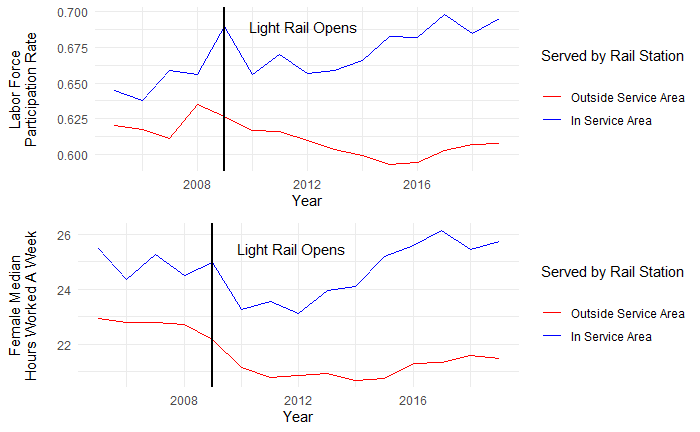
\includegraphics[width=1\textwidth]{Graphs/emp_outcomes_seattle.png}
\end{figure}
\FloatBarrier

The results of my panel event study can be shown in Figure \ref{seattle_dind}. All estimations have standard errors clustered at the PUMA level and the regression table for the estimates of these graphs can be found in Appendix \ref{appendix:tables} in Table \ref{tab:seattle_dind}. In these graphs, the y-axis is representative of the difference in employment outcomes between PUMAs served by the light rail line and the PUMAs that are not served, corresponding to the beta's in Equation (\ref{eqn}). The error bars around each estimate are set at a confidence level of 95\%. The treatment starts at $t = 0$ and all changes are compared to the "zero" date of 2008, indicated on the graphs by the dotted line.\\ 

As seen in Figure \ref{seattle_dind}, the pre-trend difference between treated and control PUMAS is not statistically significant from 0 for both the LFPR and the mean monthly hours worked for all women in the greater Seattle area, giving credence to the assumption of parallel pre-treatment test trends. In both cases, the post-treatment parallel trend does not deviate from the control trend by any statistically significant amount. After the introduction of the rapid transit system both LFPR and average hours worked began to increase slowly, with no increase being significant until 5 years after the treatment. By the 7 year mark, PUMAs that were served by the Link Light Rail System saw the LFPR and mean hours worked a week be 5.3 percentage points and 2.6 percent higher respectively when compared to the counterfactual un-treated PUMAS. The magnitude of that increase stayed relatively constant for the LFPR till the end of the sample.\\

\begin{figure}[h]
\caption{Panel Event Studies for Subsets of Women in the Seattle Area}
\label{seattle_dind}
\centering
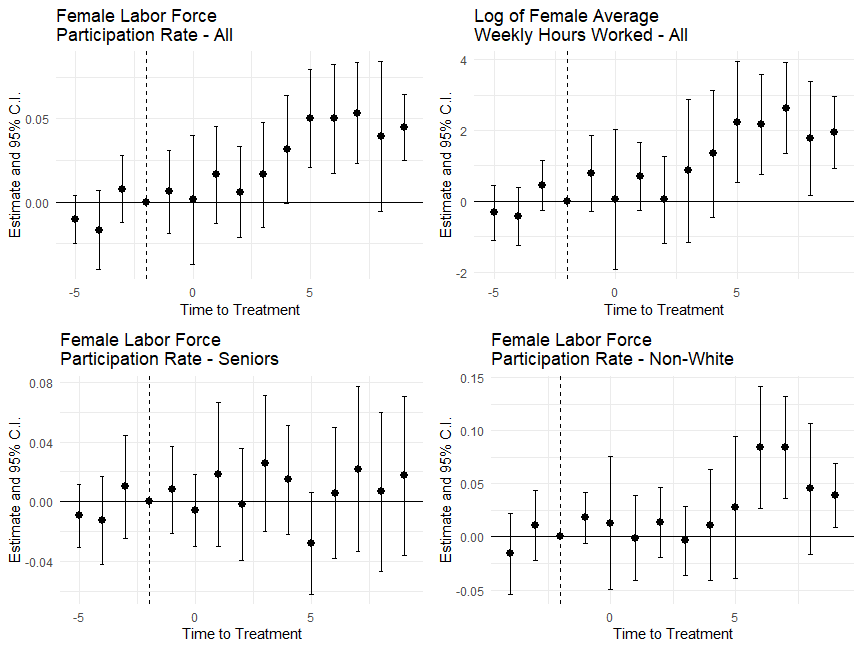
\includegraphics[width=1.0\textwidth]{Graphs/dynamic_seattle.png}
\end{figure}

As we look at the analysis on different sub-groups of the population, we see some surprising results. Although both sub-groups also have parallel pre-treatment trends, we do not observe as strong of an post-treatment effect on the LFPR on either seniors or non-white citizens. There exist some significant deviations in the post-treatment trends for minorities, it is weaker and does not have the same staying-power over time. However, the deviations that are significant have a larger difference in magnitude than the un-aggregated analysis, with the LFPR of treated PUMAs being 8.4 percentage points higher than the counterfactual. For the senior sub-group analysis, no post-treatment year trend difference was significantly different from zero.\\

\subsection{Interpretation}

In the un-aggregated panel event study regressions, I find that the opening of the Link Light Rail Line had significant increases in the employment outcomes of the women who were within the PUMAS served by the new Link Light Rail system. Five years after the opening of the system, women who lived closest to new stations had a  the labor force participation rate was 5.0 percentage points higher than the parallel counter factual would suggest. Similarly, these women also experienced a 2.2 percent increase in average hours worked per week, with both of these benefits persisting over time. The first few year after the stations opening having a negligible effect on employment outcomes is definitely of note, but it could be explained in a few ways. One is that, because transit usage is already relatively low in America, perhaps it took longer for people to understand the benefit this alternative mode of transportation could provide. Another explanation, considering specifically working hours, is that perhaps the rail line opened up more full-time job opportunities, but women just felt less secure in quitting their current job for a different one in the wage of the great recession. \\

A surprising result in my intra-city analysis is the lack of any significant change in the employment in women over the age of 65 after the opening of the rail line. This is the opposite finding of that which is found in \citeauthor{kim_subways_2019} (\citeyear{kim_subways_2019}), in which they find that senior women see stronger increases in labour outcomes compared to the general populous. Another interesting observation is the weaker effect the treatment had on non-white women comparatively. Although the effect in itself is larger in magnitude, I expected it to be more significant and with more staying power, considering non-white residents are disproportionately more likely to take transit. There could be a few reasons for this. In a PUMA that has a rail station serving it, the racial distribution of residents is most likely not homogeneous, and it could be the case that minorities have worse station access compared to the white residents within the same PUMA. It may also be the case that the additional jobs that the rail line serves are in industries and fields that historically skewed white and perhaps discriminated against minorities. Therefore, even though physical access to these jobs could have increased, the nature of said jobs could be inaccessible to minorities, providing less benefit. \\

\section{Inter-City Analysis}

\subsection{Methodology and Data}

For this paper, along with comparing PUMAs in Seattle that are served by light rail with PUMAs in Seattle that were not, I also wanted to do a analysis similar to \citeauthor{kim_subways_2019} (\citeyear{kim_subways_2019}) in where I compare the employment outcomes of Seattle before and after the subway opened with cities that already had rapid transit. As mentioned earlier, like Daejeon, Seattle was one of the last major cities in America to get a rapid transit system. Therefore, using the same general form outlined in Equation (\ref{eqn}), I will perform a panel event study comparing the employment outcomes of women in PUMAS served by rapid transit in Seattle, with the employment outcomes of women in PUMAS served by rapid transit in other metropolitan areas.  \\

The data and outcomes in this section are the same as the variables used in my intra-city analysis, just expanded to include the other American cities. Instead of comparing city wide employment outcomes like \citeauthor{kim_subways_2019} (\citeyear{kim_subways_2019}), I decide to only compare PUMAs that intersect with a 2km buffer around a rapid transit system in their respective metropolitan areas. I have chosen the latter approach over the former for two reasons. The first is that, unlike Korea, public transit usage in America is relatively low. Therefore, by focusing on only those who are served by transit, narrow the focus and reduce the noise in the data in order to see if the employment outcomes in Seattle PUMAs can "catch-up" to PUMAs already served by transit. The second reason for this approach is because the choice of where in a city to build a rapid tranist system is not exogenous to demographics or economic factors. Therefore, by comparing only the neighbourhoods that were chosen to have rapid transit, we can attempt to reduce that source of exogenous variation.\\

As I alluded to in the History of Transit in America section, choosing which cities to compare to Seattle is difficult due to the heterogeneity of American cities. In this analysis, I will first start by comparing to cities that have both second and third generation rapid transit systems. However, for robustness, I will also perform the same analysis against 2nd and 3rd generation cities separately as well. Also, I have decided to ommit any counties that saw new rapid transit stations built in their general catchment area during our period of study in order to avoid cross-shocks from other sources. \\

in this panel event study, I will be using the same control variables as were used in the intra-city event study. The standard errors will be clustered at the metropolitan area level instead of the PUMA level.\\

\subsection{Results and Interpretation}

The results of this inter-city panel event analysis is displayed in Figure \ref{gen_all} with the associated regression table in Table \ref{tab:msa_dind} in Appendix \ref{appendix:tables}. The results of this analysis is much weaker than the intra-city analysis, so I will keep this section brief.  Starting with the female labor force participation rate, although we have a parallel pre-treatment trends, we fail to see any significant positive, upward trend upwards post-treatment. In fact, the only significant deviation is at the second and third post-treatment periods where we see a relative decrease in employment compared to the constructed baseline. I have no explanation for this. \\

The relative change in average hours worked are even less significant. As there is no parallel pre-treatment trend, we cannot make any meaningful inferences from this data. We get similar insignificant events when we subset our data into comparing Seattle with just second generation cities or third generation cities, the results of which can be found in Appendix \ref{appendix:maps} in Figure \ref{fig:gen_sep}. \\

\begin{figure}[hbt!]
\caption{Trends of Employment Outcomes for Women Across Generation 2 and 3 Metro Areas}
\label{gen_all}
\centering
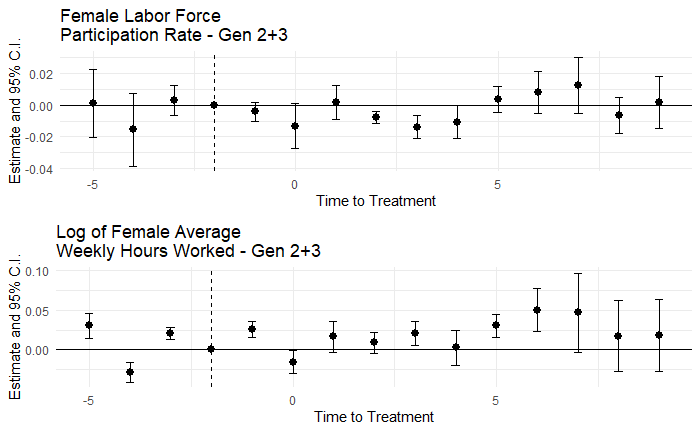
\includegraphics[width=1\textwidth]{Graphs/emp_outcome_allgen.png}
\end{figure}

\section{Discussion, Limitations, and Conclusion}

Overall, there is evidence that suggests that the opening of the Link Light Rail System was able to improve both the labor force participation rate and increase the median number of hours worked a week in the long run for women who lived relatively close to the new system. However, there are a few limitations that hinder the assumptions we can make with these results.

First and foremost is the small, relatively course PUMA levels limit the number of observations we can make. In the future, more geographically specific units of aggregation along with more temporally frequent observations would help reduce our margins of error and in turn have more accurate results. 

Another source of variation that could potentially bias my results is the inability to account how the rail line could overstate the change through secondary, unintended effects. Specifically, I have no way of testing if the increase in the LFPR is because women who live in those neighbourhoods are now able to get jobs, or if it is because women who are not in the labor force are force out of the neighbourhood due to higher rents that the presence of the light rail system induces. Therefore, although there is strong evidence that the rail line increases labor force participation rates within Seattle, this analysis has no way of implying what mechanism of the rail line is causing that change, and whether or not that change is ultimately a socially positive effect. 

Finally, I am still unsure why the intra-city analysis had such strong aggregate results, when the inter-city analysis failed to produce any positive results. Perhaps there is to much heterogeneity between American cities, or perhaps Seattle itself is just an outlier when compared to other American cities. Either way, this would be an interesting direction for further analysis. 

Ultimately, there is strong evidence to at least that rapid transit in Seattle helped improve the long term labor outcomes of women who could serve it, and that such improvements were consistant over time. 

%----------------------------------------------------
%-- APPENDIX
%----------------------------------------------------

\newpage

\section{Bibliography}
\printbibliography

\newpage

\begin{appendices}

\section{Figures and Maps Appendix}
\label{appendix:maps}

\begin{figure}[h]
\caption{Link Light Rail System in Seattle}
\label{maps:link}
\centering
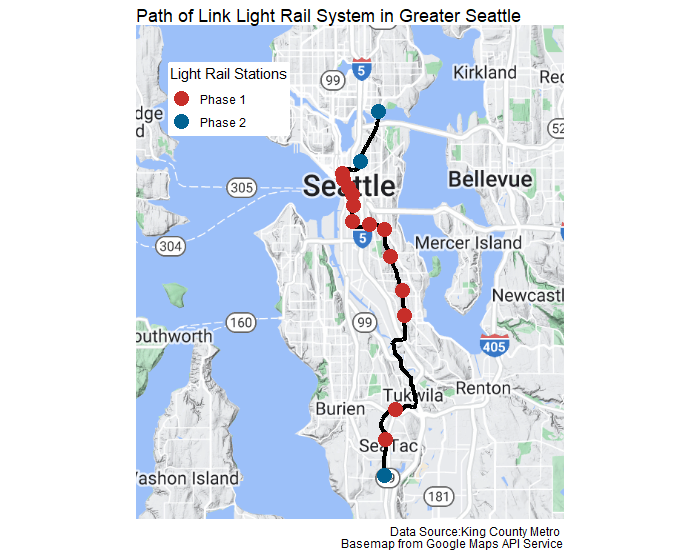
\includegraphics[width=1.0\textwidth]{Maps/link_light_rail_map.png}
\end{figure}

\begin{figure}[h]
\caption{Mode Share}
\label{maps:mode}
\centering
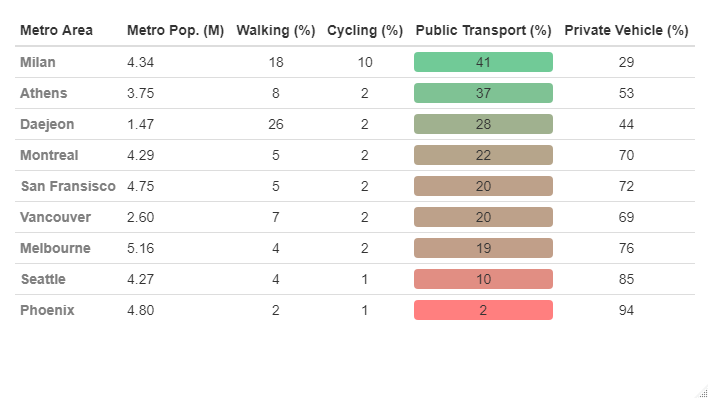
\includegraphics[width=1.0\textwidth]{Tables/mode_share.png}
\end{figure}

\begin{figure}[h]
\caption{Map of the 2500m buffers and the PUMAS They Intersect With}
\label{maps:buffer}
\centering
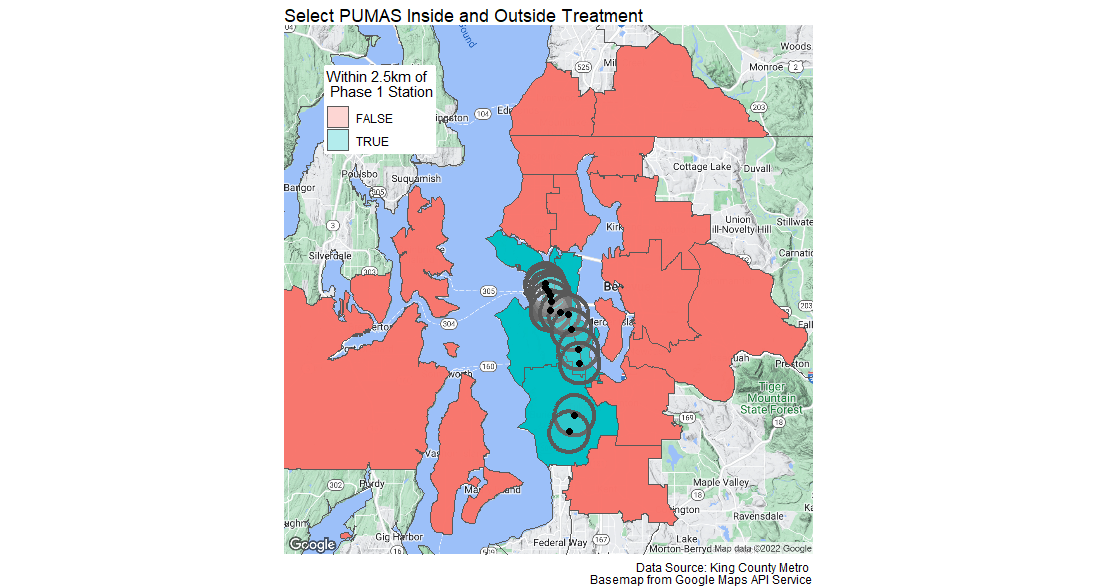
\includegraphics[width=1.0\textwidth]{Maps/PUMA_treatment_areas.png}
\end{figure}

\begin{figure}[h]
\caption{Unadjusted LFPR of Seattle vs Other Cities with Transit Systems}
\label{maps:intra}
\centering
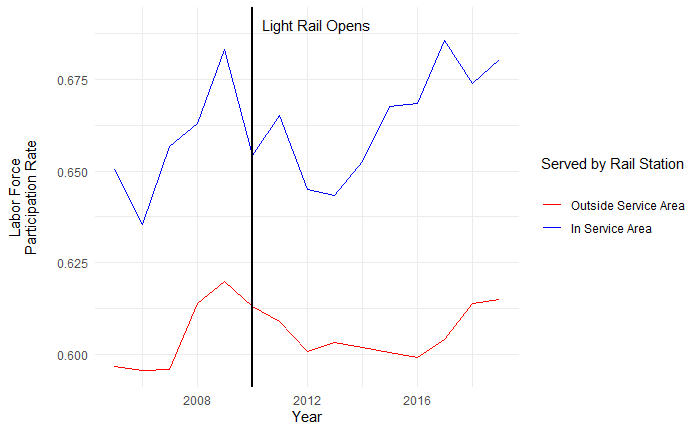
\includegraphics[width=1.0\textwidth]{Graphs/intra_graph.png}
\end{figure}

\begin{figure}[h]
\caption{Inter-city event study plots separated by Generation of system}
\label{fig:gen_sep}
\centering
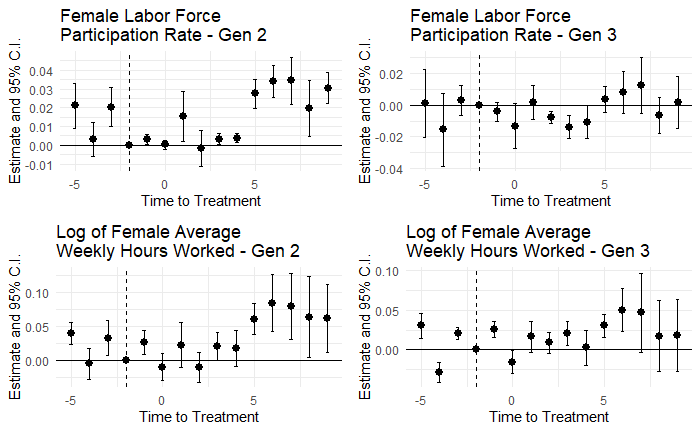
\includegraphics[width=1.0\textwidth]{Graphs/emp_outcome_gensep.png}
\end{figure}

\newpage

\section{Tables Appendix}
\label{appendix:tables}

\begin{table}[ht]
    \caption{Coefficients for all regressions in the intra-city analysis}
    \label{tab:seattle_dind}
    \centering
    \scalebox{0.78}{
    \begin{tabular}{lcccc}
    \label{seattle_dind_table}
    \tabularnewline \midrule \midrule
   Dependent Variables: & lfpr & log(hours) & senior\_lfpr & minority\_lfpr \\
   Model:                                                & (1)            & (2)           & (3)      & (4)\\  
   \midrule
   \emph{Variables}\\
   has\_station\_p1 $\times$ time\_to\_treat $=$ -5      & -0.0102        & -0.3278       & -0.0095  &   \\   
                                                         & (0.0073)       & (0.3963)      & (0.0108) &   \\   
   has\_station\_p1 $\times$ time\_to\_treat $=$ -4      & -0.0168        & -0.4289       & -0.0128  & -0.0157\\   
                                                         & (0.0121)       & (0.4121)      & (0.0151) & (0.0194)\\   
   has\_station\_p1 $\times$ time\_to\_treat $=$ -3      & 0.0076         & 0.4518        & 0.0100   & 0.0108\\   
                                                         & (0.0103)       & (0.3557)      & (0.0175) & (0.0170)\\   
   has\_station\_p1 $\times$ time\_to\_treat $=$ -1      & 0.0061         & 0.7863        & 0.0080   & 0.0181\\   
                                                         & (0.0128)       & (0.5451)      & (0.0149) & (0.0122)\\   
   has\_station\_p1 $\times$ time\_to\_treat $=$ 0       & 0.0014         & 0.0520        & -0.0061  & 0.0131\\   
                                                         & (0.0197)       & (1.010)       & (0.0123) & (0.0320)\\   
   has\_station\_p1 $\times$ time\_to\_treat $=$ 1       & 0.0164         & 0.7012        & 0.0183   & -0.0012\\   
                                                         & (0.0149)       & (0.4919)      & (0.0246) & (0.0205)\\   
   has\_station\_p1 $\times$ time\_to\_treat $=$ 2       & 0.0060         & 0.0380        & -0.0019  & 0.0133\\   
                                                         & (0.0139)       & (0.6206)      & (0.0192) & (0.0168)\\   
   has\_station\_p1 $\times$ time\_to\_treat $=$ 3       & 0.0164         & 0.8646        & 0.0256   & -0.0037\\   
                                                         & (0.0161)       & (1.032)       & (0.0234) & (0.0164)\\   
   has\_station\_p1 $\times$ time\_to\_treat $=$ 4       & 0.0315$^{*}$   & 1.342         & 0.0149   & 0.0108\\   
                                                         & (0.0164)       & (0.9121)      & (0.0186) & (0.0267)\\   
   has\_station\_p1 $\times$ time\_to\_treat $=$ 5       & 0.0502$^{***}$ & 2.229$^{**}$  & -0.0277  & 0.0275\\   
                                                         & (0.0151)       & (0.8706)      & (0.0174) & (0.0340)\\   
   has\_station\_p1 $\times$ time\_to\_treat $=$ 6       & 0.0500$^{***}$ & 2.169$^{***}$ & 0.0058   & 0.0844$^{***}$\\   
                                                         & (0.0166)       & (0.7171)      & (0.0224) & (0.0293)\\   
   has\_station\_p1 $\times$ time\_to\_treat $=$ 7       & 0.0533$^{***}$ & 2.632$^{***}$ & 0.0218   & 0.0844$^{***}$\\   
                                                         & (0.0154)       & (0.6557)      & (0.0283) & (0.0244)\\   
   has\_station\_p1 $\times$ time\_to\_treat $=$ 8       & 0.0391$^{*}$   & 1.762$^{**}$  & 0.0066   & 0.0455\\   
                                                         & (0.0229)       & (0.8205)      & (0.0272) & (0.0316)\\   
   has\_station\_p1 $\times$ time\_to\_treat $=$ 9       & 0.0449$^{***}$ & 1.942$^{***}$ & 0.0173   & 0.0390$^{**}$\\   
                                                         & (0.0102)       & (0.5241)      & (0.0273) & (0.0153)\\   
   perc\_college                                         & 0.1499$^{***}$ & 6.080$^{***}$ & -0.0216  & 0.0458\\   
                                                         & (0.0440)       & (1.960)       & (0.0587) & (0.0765)\\   
   perc\_married                                         & -0.0584        & -0.5851       & 0.0952   & -0.1731\\   
                                                         & (0.0548)       & (1.473)       & (0.0635) & (0.1026)\\   
   perc\_with\_children                                  & 0.0335         & 1.509         & 0.0063   & 0.0333\\   
                                                         & (0.0396)       & (1.810)       & (0.0469) & (0.0765)\\   
   unemp\_rate\_men                                      & -0.0603        & -6.734$^{**}$ & -0.1208  & -0.3552$^{***}$\\   
                                                         & (0.0650)       & (2.916)       & (0.0848) & (0.1238)\\   
   \midrule
   \emph{Fixed-effects}\\
   GEOID                                                 & Yes            & Yes           & Yes      & Yes\\  
   year                                                  & Yes            & Yes           & Yes      & Yes\\  
   \midrule
   \emph{Fit statistics}\\
   Observations                                          & 472            & 472           & 472      & 439\\  
   R$^2$                                                 & 0.81781        & 0.87239       & 0.30091  & 0.46831\\  
   Within R$^2$                                          & 0.16650        & 0.19805       & 0.03479  & 0.07075\\  
   \midrule \midrule
   \multicolumn{5}{l}{\emph{Clustered (GEOID) standard-errors in parentheses}}\\
   \multicolumn{5}{l}{\emph{Signif. Codes: ***: 0.01, **: 0.05, *: 0.1}}\\
\end{tabular}}
\end{table}

\begin{table}[ht]
    \caption{Coefficients for all regressions in the inter-city analysis}
    \label{tab:msa_dind}
    \centering
    \scalebox{0.78}{
    \begin{tabular}{lcccccc}
   \tabularnewline \midrule \midrule
   Dependent Variables: & \multicolumn{3}{c}{lfpr} & \multicolumn{3}{c}{log\_hours}\\
   Model:                                          & (GEN 2+3)            & (GEN 2)            & (GEN 3)            & (GEN 2+3)            & (GEN 2)            & (GEN 3)\\  
   \midrule
   \emph{Variables}\\
   is\_seattle $\times$ time\_to\_treat $=$ -5     & 0.0068         & 0.0175$^{***}$  & 0.0019                & 0.0285$^{***}$  & 0.0362$^{***}$  & 0.0362$^{***}$\\   
                                                   & (0.0055)       & (0.0041)        & (0.0072)              & (0.0048)        & (0.0051)        & (0.0051)\\   
   is\_seattle $\times$ time\_to\_treat $=$ -4     & -0.0096$^{*}$  & -0.0015         & -0.0134$^{*}$         & -0.0223$^{***}$ & -0.0115$^{*}$   & -0.0115$^{*}$\\   
                                                   & (0.0044)       & (0.0034)        & (0.0066)              & (0.0052)        & (0.0049)        & (0.0049)\\   
   is\_seattle $\times$ time\_to\_treat $=$ -3     & 0.0097$^{*}$   & 0.0209$^{***}$  & 0.0043                & 0.0225$^{***}$  & 0.0328$^{**}$   & 0.0328$^{**}$\\   
                                                   & (0.0047)       & (0.0045)        & (0.0043)              & (0.0069)        & (0.0103)        & (0.0103)\\   
   is\_seattle $\times$ time\_to\_treat $=$ -1     & 0.0021         & 0.0038$^{*}$    & 0.0025                & 0.0301$^{***}$  & 0.0282$^{**}$   & 0.0282$^{**}$\\   
                                                   & (0.0025)       & (0.0016)        & (0.0041)              & (0.0039)        & (0.0095)        & (0.0095)\\   
   is\_seattle $\times$ time\_to\_treat $=$ 0      & -0.0051        & -0.0008         & -0.0069               & -0.0094$^{**}$  & -0.0100         & -0.0100\\   
                                                   & (0.0031)       & (0.0017)        & (0.0057)              & (0.0042)        & (0.0089)        & (0.0089)\\   
   is\_seattle $\times$ time\_to\_treat $=$ 1      & 0.0091$^{**}$  & 0.0124          & 0.0073                & 0.0201$^{***}$  & 0.0207          & 0.0207\\   
                                                   & (0.0036)       & (0.0068)        & (0.0053)              & (0.0059)        & (0.0139)        & (0.0139)\\   
   is\_seattle $\times$ time\_to\_treat $=$ 2      & -0.0009        & -0.0027         & $5.06\times 10^{-5}$  & 0.0062          & -0.0092         & -0.0092\\   
                                                   & (0.0034)       & (0.0047)        & (0.0045)              & (0.0068)        & (0.0087)        & (0.0087)\\   
   is\_seattle $\times$ time\_to\_treat $=$ 3      & -0.0003        & 0.0020          & -0.0018               & 0.0291$^{***}$  & 0.0192$^{*}$    & 0.0192$^{*}$\\   
                                                   & (0.0040)       & (0.0012)        & (0.0071)              & (0.0061)        & (0.0081)        & (0.0081)\\   
   is\_seattle $\times$ time\_to\_treat $=$ 4      & 0.0027         & 0.0031          & 0.0008                & 0.0222$^{**}$   & 0.0169          & 0.0169\\   
                                                   & (0.0039)       & (0.0022)        & (0.0074)              & (0.0073)        & (0.0095)        & (0.0095)\\   
   is\_seattle $\times$ time\_to\_treat $=$ 5      & 0.0207$^{***}$ & 0.0290$^{***}$  & 0.0160$^{*}$          & 0.0532$^{***}$  & 0.0639$^{***}$  & 0.0639$^{***}$\\   
                                                   & (0.0057)       & (0.0040)        & (0.0079)              & (0.0098)        & (0.0123)        & (0.0123)\\   
   is\_seattle $\times$ time\_to\_treat $=$ 6      & 0.0223$^{***}$ & 0.0329$^{***}$  & 0.0172$^{**}$         & 0.0698$^{***}$  & 0.0864$^{***}$  & 0.0864$^{***}$\\   
                                                   & (0.0056)       & (0.0033)        & (0.0072)              & (0.0117)        & (0.0174)        & (0.0174)\\   
   is\_seattle $\times$ time\_to\_treat $=$ 7      & 0.0260$^{***}$ & 0.0363$^{***}$  & 0.0204$^{**}$         & 0.0669$^{***}$  & 0.0840$^{**}$   & 0.0840$^{**}$\\   
                                                   & (0.0068)       & (0.0060)        & (0.0080)              & (0.0163)        & (0.0222)        & (0.0222)\\   
   is\_seattle $\times$ time\_to\_treat $=$ 8      & 0.0121         & 0.0233$^{**}$   & 0.0059                & 0.0475$^{**}$   & 0.0665$^{**}$   & 0.0665$^{**}$\\   
                                                   & (0.0079)       & (0.0077)        & (0.0095)              & (0.0186)        & (0.0252)        & (0.0252)\\   
   is\_seattle $\times$ time\_to\_treat $=$ 9      & 0.0218$^{**}$  & 0.0333$^{***}$  & 0.0146                & 0.0518$^{**}$   & 0.0747$^{**}$   & 0.0747$^{**}$\\   
                                                   & (0.0073)       & (0.0037)        & (0.0102)              & (0.0192)        & (0.0265)        & (0.0265)\\   
   perc\_college                                   & 0.1791$^{***}$ & 0.0731$^{*}$    & 0.2301$^{***}$        & 0.4551$^{***}$  & 0.2460$^{***}$  & 0.2460$^{***}$\\   
                                                   & (0.0397)       & (0.0310)        & (0.0253)              & (0.0838)        & (0.0582)        & (0.0582)\\   
   perc\_married                                   & -0.0773$^{**}$ & -0.1114$^{***}$ & -0.0554               & -0.2731$^{***}$ & -0.3775$^{***}$ & -0.3775$^{***}$\\   
                                                   & (0.0323)       & (0.0241)        & (0.0644)              & (0.0719)        & (0.0612)        & (0.0612)\\   
   perc\_with\_children                            & -0.0043        & 0.0505          & 0.0040                & -0.0592         & -0.0005         & -0.0005\\   
                                                   & (0.0427)       & (0.1056)        & (0.0402)              & (0.0936)        & (0.2249)        & (0.2249)\\   
   unemp\_rate                                     & -0.0036        & -0.3003         & 0.1120                & -0.3843         & -1.043$^{***}$  & -1.043$^{***}$\\   
                                                   & (0.1250)       & (0.1591)        & (0.0617)              & (0.2484)        & (0.2365)        & (0.2365)\\   
   \midrule
   \emph{Fixed-effects}\\
   CBSAFP                                          & Yes            & Yes            & Yes            & Yes            & Yes            & Yes\\  
   year                                            & Yes            & Yes            & Yes            & Yes            & Yes            & Yes\\  
   \midrule
   \emph{Fit statistics}\\
   Observations                                    & 1,207          & 1,046          & 1,207          & 1,207          & 1,046          & 1,046\\  
   R$^2$                                           & 0.57525        & 0.56207        & 0.57525        & 0.69905        & 0.63743        & 0.63743\\  
   Within R$^2$                                    & 0.49685        & 0.14822        & 0.49685        & 0.62122        & 0.34119        & 0.34119\\  
   \midrule \midrule
   \multicolumn{7}{l}{\emph{Clustered (Metro_Area) standard-errors in parentheses}}\\
   \multicolumn{7}{l}{\emph{Signif. Codes: ***: 0.01, **: 0.05, *: 0.1}}\\
\end{tabular}}
\end{table}

\end{appendices}

\end{document}